\documentclass[12pt,letterpaper]{exam}
\usepackage[lmargin=1in,rmargin=1in,tmargin=1in,bmargin=1in]{geometry}
\usepackage{../style/exams}

% -------------------
% Course & Exam Information
% -------------------
\newcommand{\course}{MATH 141: Exam 3}
\newcommand{\term}{Fall ---\textsubscript{\textsubscript{1}} 2025}
\newcommand{\examdate}{11/21/2025}
\newcommand{\timelimit}{50 Minutes}

\setbool{hideans}{true} % Student: True; Instructor: False

\usepgfplotslibrary{fillbetween}

% -------------------
% Content
% -------------------
\begin{document}

\examtitle
\instructions{Write your name on the appropriate line on the exam cover sheet. This exam contains \numpages\ pages (including this cover page) and \numquestions\ questions. Check that you have every page of the exam. Answer the questions in the spaces provided on the question sheets. Be sure to answer every part of each question and show all your work. If you run out of room for an answer, continue on the back of the page --- being sure to indicate the problem number.} 
\scores
\bottomline
\newpage


% -------------------
% Questions
% -------------------
\begin{questions}

% Question 1
\newpage
\question Showing all your work, compute the following: \par\vspace{1cm}
	\begin{parts}
	\part[3] $\ds\int \tan \theta \;d\theta$ \psol{$=\boxed{\ln|\sec \theta| + C}= -\ln|\cos \theta| + C$} \par\vspace{2cm}
	\part[3] $\ds\int \sec \theta \;d\theta$ \psol{$= \boxed{\ln|\sec \theta + \tan \theta| + C}$} \par\vspace{2cm}
	\part[3] $\ds\int \dfrac{dx}{x^2 + 1}$ \psol{$= \boxed{\arctan x + C}$} \par\vspace{2cm}
	\part[6] $\ds\dfrac{d}{dx} \int_{\cot x}^\pi \cos(t^2) \;dt$ \pspace
	
	\vsol{\itshape Using the Fundamental Theorem of Calculus and Chain Rule, we know that if $a$ is a constant, then $\ds\dfrac{d}{dx}\, \int_a^{g(x)} f(t) \;dt= f \big( g(x) \big) \cdot g'(x)$. Using the fact that $\ds\int_a^b f(x) \;dx= -\int_b^a f(x) \;dx$, we have\dots
		\[
		\dfrac{d}{dx} \int_{\cot x}^\pi \cos(t^2) \;dt= -\dfrac{d}{dx} \int_\pi^{\cot x} \cos(t^2) \;dt= - \cos\big(\!\cot^2 x \big) \cdot (-\csc^2 x)= \boxed{\csc^2(x) \cos\big( \!\cot^2 x \big)}
		\]
	}
	\end{parts}



% Question 2
\newpage
\question[15] Below is a plot of a function $f(x)$. Showing all your work, use this plot to answer the questions below. {\itshape You may not find equations for $f(x)$.}
	\[
	\fbox{
	\begin{tikzpicture}[scale=1.3,every node/.style={scale=0.5}]
	\begin{axis}[
	grid=both,
	axis lines=middle,
	ticklabel style= {fill= blue!5!white},
	xmin= -0.5, xmax=10.5,
	ymin= -5.5, ymax=5.5,
	xtick= {-10,-8,...,10},
	ytick= {-10,-8,...,10},
	minor tick = {-10,-9,...,10},
	xlabel= \(x\), ylabel= \(y\)
	]
	\node at (7.6,2.4) {\Large$f(x)$};
	\addplot[thick, samples=2, smooth, domain= 0:5] {-3};
	\addplot[thick, samples=100, smooth, domain= 5:9] {9 - x};
	\addplot[holdot] coordinates{(5,4)};
	\addplot[soldot] coordinates{(5,-3)};
	
	\vsol{\draw[fill=red!50,opacity=0.5] (0,-3) rectangle (5,0);}
	\vsol{\draw[fill=blue!50,opacity=0.5] (5,0) -- (9,0) -- (5,4) -- (5,0);}
	\end{axis}
	\end{tikzpicture}
	}
	\] \par\vspace{0.2cm}

\begin{enumerate}[(a)]
\item $\ds\int_4^4 f(x) \;dx$ \psol{$= \boxed{0}$} \par\vspace{1.445cm}
\item $\ds\int_0^5 f(x) \;dx$ \psol{$= 5(-3)= \boxed{-15}$} \par\vspace{1.445cm}
\item $\ds\int_5^0 f(x) \;dx$ \psol{$\ds = -\int_0^5 f(x) \;dx= -(-15)= \boxed{15}$} \par\vspace{1.435cm}
\item $\ds\int_5^9 f(x) \;dx$ \psol{$= \dfrac{1}{2} \,(4)\, 4= \boxed{8}$} \par\vspace{1.31cm}
\item Find the area between $f(x)$ and the $x$-axis. \pspace
	\vsol{\itshape We want this area to be positive as we are finding the area between curves. The integral treats much of this area as negative---as it is under the $x$-axis. Therefore, we have\dots
		\[
		\text{Area}= |-15| + 8= 15 + 8= \boxed{23}
		\]
		}
\end{enumerate}



% Question 3
\newpage
\question[15] Choose \underline{\textbf{one}} of the following problems and answer it. Clearly label the part chosen and circle it. Show all your work and fully justify your reasoning. 
	\begin{enumerate}[(a)]
	\item Show that the equation $2 - e^x= 4x$ has a solution in the interval $[0, 1]$.
	\item Find the value(s), $c$, given by the Mean Value Theorem for the function $f(x)= x - x^2$ on $[-1, 5]$
	\end{enumerate} \pspace

\vsol{%
\itshape 
\begin{enumerate}[(a)]
\item Observe that\dots
	\[
	\begin{gathered}
	2 - e^x= 4x \\
	0= 4x + e^x - 2
	\end{gathered}
	\]
Let $f(x)= 4x + e^x - 2$. We know from above that the equation above has a solution on $[0, 1]$ if and only if the function $f(x)$ has a 0 on $[0, 1]$. We know that $4x$, $e^x$, and $2$ are everywhere continuous (they are polynomial, exponential, and constant functions, respectively). Therefore, $f(x)$ is everywhere continuous because it is the sum/difference of continuous functions. So, $f(x)$ is continuous on $[0, 1]$. But\dots
	\[
	\begin{aligned}
	f(0)&= 4(0) + e^0 - 2= 0 + 1 - 2= -1 < 0\\
	f(1)&= 4(1) + e^1 - 2= 4 + e - 2= 2 + e > 0
	\end{aligned}
	\]
But then $f(0) < 0 < f(1)$. By the Intermediate Value Theorem, there exists $c \in (0, 1)$ such that $f(c)= 0$. But then $0= 4c + e^c - 2$, i.e. $2 - e^c= 4c$. Therefore, the equation $2 - e^x= 4x$ has a solution in the interval $[0, 1]$. [In fact, $c \approx 0.19589899188683166$.] \pspace

\item The function $f(x)= x - x^2$ is a polynomial and therefore everywhere continuous and differentiable. So, $f(x)$ is continuous on $[-1, 5]$ and differentiable on $(-1, 5)$. Therefore, by the Mean Value Theorem, there exists $c \in (-1, 5)$ such that $f'(c)= \frac{f(5) - f(-1)}{5 - (-1)}$, i.e. so that moment the instantaneous rate is the average rate. We have\dots
	\[
	\begin{aligned}
	f'(x)&= 1 - 2x \\[0.2cm]
	f(5)&= 5 - 5^2= 5 - 25= -20 \\[0.2cm]
	f(-1)&= -1 - (-1)^2= -1 - 1= -2 \\[0.2cm]
	\frac{f(5) - f(-1)}{5 - (-1)}&= \dfrac{-20 - (-2)}{5 + 1}= \dfrac{-18}{6}= -3
	\end{aligned}
	\]
But then we know that\dots
	\[
	\begin{gathered}
	f'(c)= \frac{f(5) - f(-1)}{5 - (-1)} \\[0.2cm]
	1 - 2c= -3 \\[0.2cm]
	2c= 4 \\[0.2cm]
	\boxed{c= 2}
	\end{gathered}
	\]
\end{enumerate}
}



% Question 4
\newpage
\question[15] Below is a plot of a function $f(x)$. Estimate $\ds\int_1^9 f(x) \;dx$ using a midpoint sum with four equally spaced rectangles. 
	\[
	\fbox{
	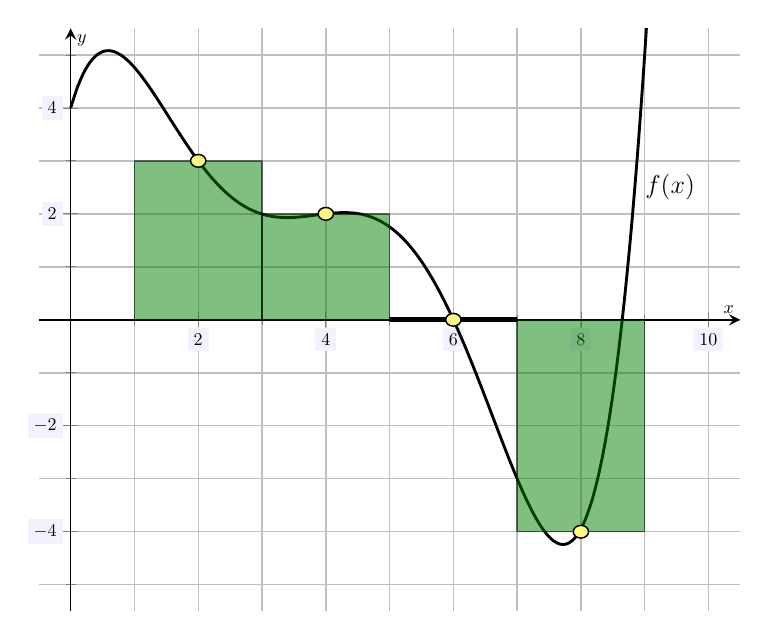
\begin{tikzpicture}[scale=1.3,every node/.style={scale=0.5}]
	\begin{axis}[
	grid=both,
	axis lines=middle,
	ticklabel style= {fill= blue!5!white},
	xmin= -0.5, xmax=10.5,
	ymin= -5.5, ymax= 5.5,
	xtick= {-10,-8,...,10},
	ytick= {-10,-8,...,10},
	minor tick = {-10,-9,...,10},
	xlabel= \(x\), ylabel= \(y\)
	]
	\node at (9.4,2.5) {\Large$f(x)$};
	\addplot[thick, samples=100, smooth, domain= 0:10] {4. + 4.17778*x - 4.92209*x^2 + 1.7461*x^3 - 0.252513*x^4 + 
 0.0126323*x^5};
 
	\vsol{\draw[fill=black!50!green,opacity=0.5] (1,0) rectangle (3,3);}
	\vsol{\draw[fill=black!50!green,opacity=0.5] (3,0) rectangle (5,2);}
	\vsol{\draw[line width=0.05cm] (5,0) rectangle (7,0);}
	\vsol{\draw[fill=black!50!green,opacity=0.5] (7,0) rectangle (9,-4);}
	\vsol{\draw[fill=white!50!yellow] (2,3) circle (0.12);}
	\vsol{\draw[fill=white!50!yellow] (4,2) circle (0.12);}
	\vsol{\draw[fill=white!50!yellow] (6,0) circle (0.12);}
	\vsol{\draw[fill=white!50!yellow] (8,-4) circle (0.12);}
	\end{axis}
	\end{tikzpicture}
	}
	\] \pspace

\vsol{\itshape If we use four equally spaced rectangles, the width of each rectangle will be $\Delta x= \dfrac{b - a}{n}= \dfrac{9 - 1}{4}= \dfrac{8}{4}= 2$. The first rectangle will begin at $x= 1$ and the last rectangle end at $x= 9$. So, we have intervals $[1, 3]$, $[3, 5]$, $[5, 7]$, and $[7, 9]$. As we are using a midpoint sum, we choose the midpoint of each of these intervals, i.e. $x= 2, 4, 6, 8$. The heights of our rectangles will be given by $f(2), f(4), f(6), f(8)$---which can be read off the graph. Therefore, we have\dots
	\[
	\begin{aligned}
	\int_1^9 f(x) \;dx&\approx \sum_{i=0}^3 f(2 + i \Delta x) \Delta x \\[0.2cm]
	&= f(2) \cdot 2 + f(4) \cdot 2 + f(6) \cdot 2 + f(8) \cdot 2 \\[0.2cm]
	&= 3 \cdot 2 + 2 \cdot 2 + 0 \cdot 2 + -4 \cdot 2 \\[0.2cm]
	&= 6 + 4 + 0 + (-8) \\[0.2cm]
	&= \boxed{2}
	\end{aligned}
	\] \vfill

{\footnotesize Note. The actual value of the integral is approximately $5.095$.}
}



% Question 5
\newpage
\question[15] Showing all your work, compute the following: \par\vspace{0.3cm}
	\begin{enumerate}[(a)]
	\item $\ds\int \left( \sin x - \dfrac{1}{x^{3/2}} + \dfrac{3}{x} \right) \;dx$ \par\vspace{1cm}
	
	\wsol{%
		\[
		\begin{aligned}
		\hspace{-3.7cm} \int \left( \sin x - \dfrac{1}{x^{3/2}} + \dfrac{3}{x} \right) \;dx&= \int \left( \sin x - x^{-3/2} + \dfrac{3}{x} \right) \;dx \\[0.3cm]
		&= -\cos x - (-2) x^{-1/2} + 3\ln|x| + C \\[0.3cm]
		&= \boxed{-\cos x+ \dfrac{2}{\sqrt{x}} + 3\ln|x| + C}
		\end{aligned}
		\]
	} \par\vspace{1cm}
	
	\item $\ds\int_{-1}^1 (1 - x^3) \;dx$ \par\vspace{1.5cm}
	
	\wsol{%
		\[
		\int_{-1}^1 (1 - x^3) \;dx= x - \dfrac{x^4}{4} \bigg|_{-1}^1= \left(1 - \dfrac{1}{4} \right) - \left(-1 - \dfrac{1}{4} \right)= 1 - \dfrac{1}{4} + 1 + \dfrac{1}{4}= \boxed{2}
		\]
	} \par\vspace{2.35cm}
	
	\item $\ds\int \sec(x) \, \big( \sec x + \tan x \big) \;dx$ \par\vspace{1.2cm}
	
	\wsol{%
		\[
		\int \sec(x) \, \big( \sec x + \tan x \big) \;dx= \int \big( \sec^2(x) + \sec x \tan x \big) \;dx= \boxed{\tan x + \sec x + C}
		\]
	}
	\end{enumerate}



% Question 6
\newpage
\question[15] A region $\mathcal{R}$ bound by the curves $y= \frac{1}{2}\, x^2$, $y= 8x$, and $y= 8$ is shaded in the figure below. 
	\[
	\fbox{
	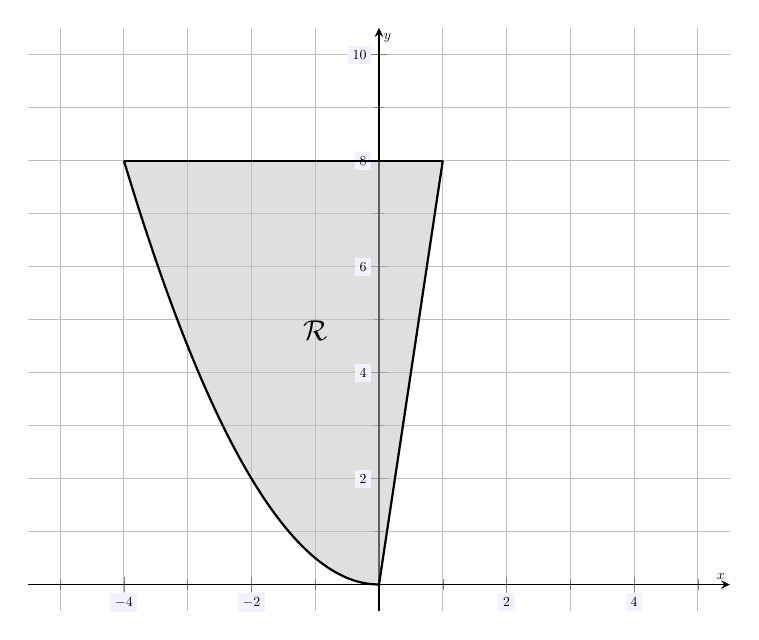
\begin{tikzpicture}[scale=1.3,every node/.style={scale=0.5}]
	\begin{axis}[
	grid=both,
	axis lines=middle,
	ticklabel style= {fill= blue!5!white},
	xmin= -5.5, xmax=5.5,
	ymin= -0.5, ymax= 10.5,
	xtick= {-6,-4,...,6},
	ytick= {-2,0,...,12},
	minor tick = {-5,-4,...,10},
	xlabel= \(x\), ylabel= \(y\)
	]
	\addplot[name path = P, thick, smooth, domain= -4:0] {1/2*x^2};
	\addplot[name path = L, thick, smooth, domain= 0:1] {8*x};
	\addplot[name path = H, thick,smooth, domain= -4:1] {8};
	\addplot[color=gray!50,opacity=0.5] fill between[of=H and P];
	\node at (-1,4.8) {\huge$\mathcal{R}$};
	\end{axis}
	\end{tikzpicture}
	}
	\]

\begin{enumerate}[(a)]
\item Set up \textit{\bfseries but do not evaluate or simplify} an integral expression \textit{\bfseries with respect to $x$} that computes the area of $\mathcal{R}$. \par\vspace{1cm}

	\wsol{%
	\[
	\boxed{\int_{-4}^0 \left( 8 - \frac{1}{2}\, x^2 \right) \;dx + \int_0^1 \left( 8 - 8x \right) \;dx}
	\]
	} \par\vspace{2.55cm}

\item Set up \textit{\bfseries but do not evaluate or simplify} an integral expression \textit{\bfseries with respect to $y$} that computes the area of $\mathcal{R}$. \par\vspace{1cm}
	
	\wsol{%
	\[
	\boxed{\int_0^8 \left( \dfrac{y}{8} - (-\sqrt{2y}\, ) \right) \;dy}
	\]
	}
\end{enumerate}

\end{questions}
\end{document}